\documentclass[1p]{elsarticle_modified}
%\bibliographystyle{elsarticle-num}

%\usepackage[colorlinks]{hyperref}
%\usepackage{abbrmath_seonhwa} %\Abb, \Ascr, \Acal ,\Abf, \Afrak
\usepackage{amsfonts}
\usepackage{amssymb}
\usepackage{amsmath}
\usepackage{amsthm}
\usepackage{scalefnt}
\usepackage{amsbsy}
\usepackage{kotex}
\usepackage{caption}
\usepackage{subfig}
\usepackage{color}
\usepackage{graphicx}
\usepackage{xcolor} %% white, black, red, green, blue, cyan, magenta, yellow
\usepackage{float}
\usepackage{setspace}
\usepackage{hyperref}

\usepackage{tikz}
\usetikzlibrary{arrows}

\usepackage{multirow}
\usepackage{array} % fixed length table
\usepackage{hhline}

%%%%%%%%%%%%%%%%%%%%%
\makeatletter
\renewcommand*\env@matrix[1][\arraystretch]{%
	\edef\arraystretch{#1}%
	\hskip -\arraycolsep
	\let\@ifnextchar\new@ifnextchar
	\array{*\c@MaxMatrixCols c}}
\makeatother %https://tex.stackexchange.com/questions/14071/how-can-i-increase-the-line-spacing-in-a-matrix
%%%%%%%%%%%%%%%

\usepackage[normalem]{ulem}

\newcommand{\msout}[1]{\ifmmode\text{\sout{\ensuremath{#1}}}\else\sout{#1}\fi}
%SOURCE: \msout is \stkout macro in https://tex.stackexchange.com/questions/20609/strikeout-in-math-mode

\newcommand{\cancel}[1]{
	\ifmmode
	{\color{red}\msout{#1}}
	\else
	{\color{red}\sout{#1}}
	\fi
}

\newcommand{\add}[1]{
	{\color{blue}\uwave{#1}}
}

\newcommand{\replace}[2]{
	\ifmmode
	{\color{red}\msout{#1}}{\color{blue}\uwave{#2}}
	\else
	{\color{red}\sout{#1}}{\color{blue}\uwave{#2}}
	\fi
}

\newcommand{\Sol}{\mathcal{S}} %segment
\newcommand{\D}{D} %diagram
\newcommand{\A}{\mathcal{A}} %arc


%%%%%%%%%%%%%%%%%%%%%%%%%%%%%5 test

\def\sl{\operatorname{\textup{SL}}(2,\Cbb)}
\def\psl{\operatorname{\textup{PSL}}(2,\Cbb)}
\def\quan{\mkern 1mu \triangleright \mkern 1mu}

\theoremstyle{definition}
\newtheorem{thm}{Theorem}[section]
\newtheorem{prop}[thm]{Proposition}
\newtheorem{lem}[thm]{Lemma}
\newtheorem{ques}[thm]{Question}
\newtheorem{cor}[thm]{Corollary}
\newtheorem{defn}[thm]{Definition}
\newtheorem{exam}[thm]{Example}
\newtheorem{rmk}[thm]{Remark}
\newtheorem{alg}[thm]{Algorithm}

\newcommand{\I}{\sqrt{-1}}
\begin{document}

%\begin{frontmatter}
%
%\title{Boundary parabolic representations of knots up to 8 crossings}
%
%%% Group authors per affiliation:
%\author{Yunhi Cho} 
%\address{Department of Mathematics, University of Seoul, Seoul, Korea}
%\ead{yhcho@uos.ac.kr}
%
%
%\author{Seonhwa Kim} %\fnref{s_kim}}
%\address{Center for Geometry and Physics, Institute for Basic Science, Pohang, 37673, Korea}
%\ead{ryeona17@ibs.re.kr}
%
%\author{Hyuk Kim}
%\address{Department of Mathematical Sciences, Seoul National University, Seoul 08826, Korea}
%\ead{hyukkim@snu.ac.kr}
%
%\author{Seokbeom Yoon}
%\address{Department of Mathematical Sciences, Seoul National University, Seoul, 08826,  Korea}
%\ead{sbyoon15@snu.ac.kr}
%
%\begin{abstract}
%We find all boundary parabolic representation of knots up to 8 crossings.
%
%\end{abstract}
%\begin{keyword}
%    \MSC[2010] 57M25 
%\end{keyword}
%
%\end{frontmatter}

%\linenumbers
%\tableofcontents
%
\newcommand\colored[1]{\textcolor{white}{\rule[-0.35ex]{0.8em}{1.4ex}}\kern-0.8em\color{red} #1}%
%\newcommand\colored[1]{\textcolor{white}{ #1}\kern-2.17ex	\textcolor{white}{ #1}\kern-1.81ex	\textcolor{white}{ #1}\kern-2.15ex\color{red}#1	}

{\Large $\underline{11a_{138}~(K11a_{138})}$}

\setlength{\tabcolsep}{10pt}
\renewcommand{\arraystretch}{1.6}
\vspace{1cm}\begin{tabular}{m{100pt}>{\centering\arraybackslash}m{274pt}}
\multirow{5}{120pt}{
	\centering
	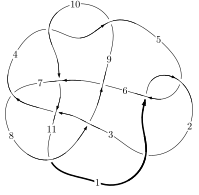
\includegraphics[width=112pt]{../../../GIT/diagram.site/Diagrams/png/387_11a_138.png}\\
\ \ \ A knot diagram\footnotemark}&
\allowdisplaybreaks
\textbf{Linearized knot diagam} \\
\cline{2-2}
 &
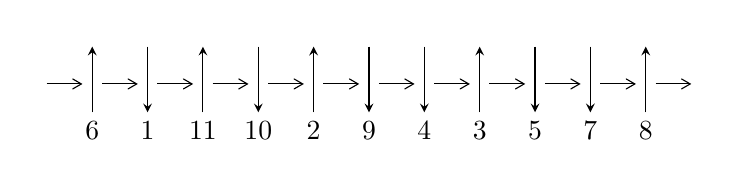
\begin{tikzpicture}[x=20pt, y=17pt]
	% nodes
	\node (C0) at (0, 0) {};
	\node (C1) at (1, 0) {};
	\node (C1U) at (1, +1) {};
	\node (C1D) at (1, -1) {6};

	\node (C2) at (2, 0) {};
	\node (C2U) at (2, +1) {};
	\node (C2D) at (2, -1) {1};

	\node (C3) at (3, 0) {};
	\node (C3U) at (3, +1) {};
	\node (C3D) at (3, -1) {11};

	\node (C4) at (4, 0) {};
	\node (C4U) at (4, +1) {};
	\node (C4D) at (4, -1) {10};

	\node (C5) at (5, 0) {};
	\node (C5U) at (5, +1) {};
	\node (C5D) at (5, -1) {2};

	\node (C6) at (6, 0) {};
	\node (C6U) at (6, +1) {};
	\node (C6D) at (6, -1) {9};

	\node (C7) at (7, 0) {};
	\node (C7U) at (7, +1) {};
	\node (C7D) at (7, -1) {4};

	\node (C8) at (8, 0) {};
	\node (C8U) at (8, +1) {};
	\node (C8D) at (8, -1) {3};

	\node (C9) at (9, 0) {};
	\node (C9U) at (9, +1) {};
	\node (C9D) at (9, -1) {5};

	\node (C10) at (10, 0) {};
	\node (C10U) at (10, +1) {};
	\node (C10D) at (10, -1) {7};

	\node (C11) at (11, 0) {};
	\node (C11U) at (11, +1) {};
	\node (C11D) at (11, -1) {8};
	\node (C12) at (12, 0) {};

	% arrows
	\draw[->,>={angle 60}]
	(C0) edge (C1) (C1) edge (C2) (C2) edge (C3) (C3) edge (C4) (C4) edge (C5) (C5) edge (C6) (C6) edge (C7) (C7) edge (C8) (C8) edge (C9) (C9) edge (C10) (C10) edge (C11) (C11) edge (C12) ;	\draw[->,>=stealth]
	(C1D) edge (C1U) (C2U) edge (C2D) (C3D) edge (C3U) (C4U) edge (C4D) (C5D) edge (C5U) (C6U) edge (C6D) (C7U) edge (C7D) (C8D) edge (C8U) (C9U) edge (C9D) (C10U) edge (C10D) (C11D) edge (C11U) ;
	\end{tikzpicture} \\
\hhline{~~} \\& 
\textbf{Solving Sequence} \\ \cline{2-2} 
 &
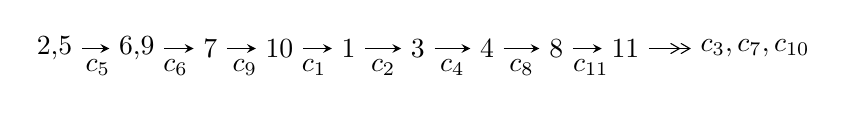
\begin{tikzpicture}[x=25pt, y=7pt]
	% node
	\node (A0) at (-1/8, 0) {2,5};
	\node (A1) at (17/16, 0) {6,9};
	\node (A2) at (17/8, 0) {7};
	\node (A3) at (25/8, 0) {10};
	\node (A4) at (33/8, 0) {1};
	\node (A5) at (41/8, 0) {3};
	\node (A6) at (49/8, 0) {4};
	\node (A7) at (57/8, 0) {8};
	\node (A8) at (65/8, 0) {11};
	\node (C1) at (1/2, -1) {$c_{5}$};
	\node (C2) at (13/8, -1) {$c_{6}$};
	\node (C3) at (21/8, -1) {$c_{9}$};
	\node (C4) at (29/8, -1) {$c_{1}$};
	\node (C5) at (37/8, -1) {$c_{2}$};
	\node (C6) at (45/8, -1) {$c_{4}$};
	\node (C7) at (53/8, -1) {$c_{8}$};
	\node (C8) at (61/8, -1) {$c_{11}$};
	\node (A9) at (10, 0) {$c_{3},c_{7},c_{10}$};

	% edge
	\draw[->,>=stealth]	
	(A0) edge (A1) (A1) edge (A2) (A2) edge (A3) (A3) edge (A4) (A4) edge (A5) (A5) edge (A6) (A6) edge (A7) (A7) edge (A8) ;
	\draw[->>,>={angle 60}]	
	(A8) edge (A9);
\end{tikzpicture} \\ 

\end{tabular} \\

\footnotetext{
The image of knot diagram is generated by the software ``\textbf{Draw programme}" developed by Andrew Bartholomew(\url{http://www.layer8.co.uk/maths/draw/index.htm\#Running-draw}), where we modified some parts for our purpose(\url{https://github.com/CATsTAILs/LinksPainter}).
}\phantom \\ \newline 
\centering \textbf{Ideals for irreducible components\footnotemark of $X_{\text{par}}$} 
 
\begin{align*}
I^u_{1}&=\langle 
4.64020\times10^{132} u^{93}-4.93260\times10^{132} u^{92}+\cdots+3.94596\times10^{132} b+2.57397\times10^{133},\\
\phantom{I^u_{1}}&\phantom{= \langle  }5.66772\times10^{133} u^{93}+4.81293\times10^{132} u^{92}+\cdots+7.49732\times10^{133} a+2.94172\times10^{134},\\
\phantom{I^u_{1}}&\phantom{= \langle  }u^{94}+18 u^{92}+\cdots+86 u+19\rangle \\
I^u_{2}&=\langle 
u^{13}+u^{12}+4 u^{11}+5 u^{10}+9 u^9+12 u^8+14 u^7+18 u^6+14 u^5+16 u^4+10 u^3+7 u^2+b+3 u+2,\\
\phantom{I^u_{2}}&\phantom{= \langle  }2 u^{11}+u^{10}+6 u^9+3 u^8+10 u^7+6 u^6+11 u^5+6 u^4+5 u^3+u^2+a+2 u,\\
\phantom{I^u_{2}}&\phantom{= \langle  }u^{14}+u^{13}+4 u^{12}+4 u^{11}+9 u^{10}+9 u^9+14 u^8+13 u^7+14 u^6+11 u^5+10 u^4+6 u^3+4 u^2+2 u+1\rangle \\
\\
\end{align*}
\raggedright * 2 irreducible components of $\dim_{\mathbb{C}}=0$, with total 108 representations.\\
\footnotetext{All coefficients of polynomials are rational numbers. But the coefficients are sometimes approximated in decimal forms when there is not enough margin.}
\newpage
\renewcommand{\arraystretch}{1}
\centering \section*{I. $I^u_{1}= \langle 4.64\times10^{132} u^{93}-4.93\times10^{132} u^{92}+\cdots+3.95\times10^{132} b+2.57\times10^{133},\;5.67\times10^{133} u^{93}+4.81\times10^{132} u^{92}+\cdots+7.50\times10^{133} a+2.94\times10^{134},\;u^{94}+18 u^{92}+\cdots+86 u+19 \rangle$}
\flushleft \textbf{(i) Arc colorings}\\
\begin{tabular}{m{7pt} m{180pt} m{7pt} m{180pt} }
\flushright $a_{2}=$&$\begin{pmatrix}0\\u\end{pmatrix}$ \\
\flushright $a_{5}=$&$\begin{pmatrix}1\\0\end{pmatrix}$ \\
\flushright $a_{6}=$&$\begin{pmatrix}1\\- u^2\end{pmatrix}$ \\
\flushright $a_{9}=$&$\begin{pmatrix}-0.755966 u^{93}-0.0641953 u^{92}+\cdots-15.1145 u-3.92369\\-1.17594 u^{93}+1.25004 u^{92}+\cdots-56.7451 u-6.52306\end{pmatrix}$ \\
\flushright $a_{7}=$&$\begin{pmatrix}-2.28733 u^{93}+2.35688 u^{92}+\cdots-121.002 u-13.5839\\1.36980 u^{93}-1.75146 u^{92}+\cdots-20.3031 u-19.9674\end{pmatrix}$ \\
\flushright $a_{10}=$&$\begin{pmatrix}0.419971 u^{93}-1.31423 u^{92}+\cdots+41.6306 u+2.59936\\-1.17594 u^{93}+1.25004 u^{92}+\cdots-56.7451 u-6.52306\end{pmatrix}$ \\
\flushright $a_{1}=$&$\begin{pmatrix}- u\\u^3+u\end{pmatrix}$ \\
\flushright $a_{3}=$&$\begin{pmatrix}- u^3\\u^5+u^3+u\end{pmatrix}$ \\
\flushright $a_{4}=$&$\begin{pmatrix}1.02372 u^{93}+2.01186 u^{92}+\cdots+240.302 u+51.4766\\2.60768 u^{93}-0.842489 u^{92}+\cdots+189.866 u+42.1854\end{pmatrix}$ \\
\flushright $a_{8}=$&$\begin{pmatrix}-1.25959 u^{93}-0.266213 u^{92}+\cdots-77.3471 u-18.8004\\-1.08401 u^{93}+1.21540 u^{92}+\cdots-51.7820 u-4.28835\end{pmatrix}$ \\
\flushright $a_{11}=$&$\begin{pmatrix}-2.05177 u^{93}+1.06053 u^{92}+\cdots-195.102 u-45.8558\\1.21606 u^{93}-0.797164 u^{92}+\cdots+40.0767 u-1.76508\end{pmatrix}$\\ \flushright $a_{11}=$&$\begin{pmatrix}-2.05177 u^{93}+1.06053 u^{92}+\cdots-195.102 u-45.8558\\1.21606 u^{93}-0.797164 u^{92}+\cdots+40.0767 u-1.76508\end{pmatrix}$\\&\end{tabular}
\flushleft \textbf{(ii) Obstruction class $= -1$}\\~\\
\flushleft \textbf{(iii) Cusp Shapes $= -17.7102 u^{93}+16.3821 u^{92}+\cdots-633.419 u-58.7338$}\\~\\
\newpage\renewcommand{\arraystretch}{1}
\flushleft \textbf{(iv) u-Polynomials at the component}\newline \\
\begin{tabular}{m{50pt}|m{274pt}}
Crossings & \hspace{64pt}u-Polynomials at each crossing \\
\hline $$\begin{aligned}c_{1},c_{5}\end{aligned}$$&$\begin{aligned}
&u^{94}+18 u^{92}+\cdots-86 u+19
\end{aligned}$\\
\hline $$\begin{aligned}c_{2}\end{aligned}$$&$\begin{aligned}
&u^{94}+36 u^{93}+\cdots+8108 u+361
\end{aligned}$\\
\hline $$\begin{aligned}c_{3}\end{aligned}$$&$\begin{aligned}
&u^{94}+5 u^{93}+\cdots+88 u+11
\end{aligned}$\\
\hline $$\begin{aligned}c_{4},c_{9}\end{aligned}$$&$\begin{aligned}
&u^{94}- u^{93}+\cdots-724 u+59
\end{aligned}$\\
\hline $$\begin{aligned}c_{6}\end{aligned}$$&$\begin{aligned}
&u^{94}+u^{93}+\cdots+33 u+781
\end{aligned}$\\
\hline $$\begin{aligned}c_{7}\end{aligned}$$&$\begin{aligned}
&u^{94}+3 u^{93}+\cdots-872 u+184
\end{aligned}$\\
\hline $$\begin{aligned}c_{8}\end{aligned}$$&$\begin{aligned}
&u^{94}- u^{93}+\cdots+6 u+1
\end{aligned}$\\
\hline $$\begin{aligned}c_{10}\end{aligned}$$&$\begin{aligned}
&u^{94}-2 u^{93}+\cdots-22 u+1
\end{aligned}$\\
\hline $$\begin{aligned}c_{11}\end{aligned}$$&$\begin{aligned}
&u^{94}-3 u^{93}+\cdots+519 u+19
\end{aligned}$\\
\hline
\end{tabular}\\~\\
\newpage\renewcommand{\arraystretch}{1}
\flushleft \textbf{(v) Riley Polynomials at the component}\newline \\
\begin{tabular}{m{50pt}|m{274pt}}
Crossings & \hspace{64pt}Riley Polynomials at each crossing \\
\hline $$\begin{aligned}c_{1},c_{5}\end{aligned}$$&$\begin{aligned}
&y^{94}+36 y^{93}+\cdots+8108 y+361
\end{aligned}$\\
\hline $$\begin{aligned}c_{2}\end{aligned}$$&$\begin{aligned}
&y^{94}+48 y^{93}+\cdots+13235584 y+130321
\end{aligned}$\\
\hline $$\begin{aligned}c_{3}\end{aligned}$$&$\begin{aligned}
&y^{94}+9 y^{93}+\cdots+7084 y+121
\end{aligned}$\\
\hline $$\begin{aligned}c_{4},c_{9}\end{aligned}$$&$\begin{aligned}
&y^{94}+69 y^{93}+\cdots-23148 y+3481
\end{aligned}$\\
\hline $$\begin{aligned}c_{6}\end{aligned}$$&$\begin{aligned}
&y^{94}+27 y^{93}+\cdots+20468921 y+609961
\end{aligned}$\\
\hline $$\begin{aligned}c_{7}\end{aligned}$$&$\begin{aligned}
&y^{94}+23 y^{93}+\cdots+1507232 y+33856
\end{aligned}$\\
\hline $$\begin{aligned}c_{8}\end{aligned}$$&$\begin{aligned}
&y^{94}-5 y^{93}+\cdots-10 y+1
\end{aligned}$\\
\hline $$\begin{aligned}c_{10}\end{aligned}$$&$\begin{aligned}
&y^{94}+8 y^{93}+\cdots-18 y+1
\end{aligned}$\\
\hline $$\begin{aligned}c_{11}\end{aligned}$$&$\begin{aligned}
&y^{94}-15 y^{93}+\cdots-72597 y+361
\end{aligned}$\\
\hline
\end{tabular}\\~\\
\newpage\flushleft \textbf{(vi) Complex Volumes and Cusp Shapes}
$$\begin{array}{c|c|c}  
\text{Solutions to }I^u_{1}& \I (\text{vol} + \sqrt{-1}CS) & \text{Cusp shape}\\
 \hline 
\begin{aligned}
u &= \phantom{-}0.772806 + 0.634311 I \\
a &= \phantom{-}0.654406 - 0.353128 I \\
b &= \phantom{-}0.323430 + 1.127770 I\end{aligned}
 & \phantom{-}2.72382 - 3.59329 I & \phantom{-0.000000 } 0 \\ \hline\begin{aligned}
u &= \phantom{-}0.772806 - 0.634311 I \\
a &= \phantom{-}0.654406 + 0.353128 I \\
b &= \phantom{-}0.323430 - 1.127770 I\end{aligned}
 & \phantom{-}2.72382 + 3.59329 I & \phantom{-0.000000 } 0 \\ \hline\begin{aligned}
u &= \phantom{-}0.274173 + 0.962209 I \\
a &= -1.50690 - 0.97979 I \\
b &= -0.396852 + 0.187929 I\end{aligned}
 & -4.34588 + 0.86890 I & \phantom{-0.000000 } 0 \\ \hline\begin{aligned}
u &= \phantom{-}0.274173 - 0.962209 I \\
a &= -1.50690 + 0.97979 I \\
b &= -0.396852 - 0.187929 I\end{aligned}
 & -4.34588 - 0.86890 I & \phantom{-0.000000 } 0 \\ \hline\begin{aligned}
u &= -0.668968 + 0.720659 I \\
a &= \phantom{-}1.016990 - 0.259896 I \\
b &= \phantom{-}0.775819 + 0.307672 I\end{aligned}
 & \phantom{-}0.151749 - 0.477282 I & \phantom{-0.000000 } 0 \\ \hline\begin{aligned}
u &= -0.668968 - 0.720659 I \\
a &= \phantom{-}1.016990 + 0.259896 I \\
b &= \phantom{-}0.775819 - 0.307672 I\end{aligned}
 & \phantom{-}0.151749 + 0.477282 I & \phantom{-0.000000 } 0 \\ \hline\begin{aligned}
u &= -0.850683 + 0.581825 I \\
a &= \phantom{-}0.246185 - 0.369614 I \\
b &= -0.406184 + 0.185472 I\end{aligned}
 & \phantom{-}1.11160 - 3.31196 I & \phantom{-0.000000 } 0 \\ \hline\begin{aligned}
u &= -0.850683 - 0.581825 I \\
a &= \phantom{-}0.246185 + 0.369614 I \\
b &= -0.406184 - 0.185472 I\end{aligned}
 & \phantom{-}1.11160 + 3.31196 I & \phantom{-0.000000 } 0 \\ \hline\begin{aligned}
u &= -0.592379 + 0.857518 I \\
a &= -1.82681 + 0.35619 I \\
b &= -0.07407 - 1.92793 I\end{aligned}
 & \phantom{-}2.76989 - 2.34388 I & \phantom{-0.000000 } 0 \\ \hline\begin{aligned}
u &= -0.592379 - 0.857518 I \\
a &= -1.82681 - 0.35619 I \\
b &= -0.07407 + 1.92793 I\end{aligned}
 & \phantom{-}2.76989 + 2.34388 I & \phantom{-0.000000 } 0\\
 \hline 
 \end{array}$$\newpage$$\begin{array}{c|c|c}  
\text{Solutions to }I^u_{1}& \I (\text{vol} + \sqrt{-1}CS) & \text{Cusp shape}\\
 \hline 
\begin{aligned}
u &= \phantom{-}0.695476 + 0.779469 I \\
a &= -0.0831373 - 0.0411398 I \\
b &= \phantom{-}0.49756 + 1.48450 I\end{aligned}
 & \phantom{-}6.51815 - 3.45234 I & \phantom{-0.000000 } 0 \\ \hline\begin{aligned}
u &= \phantom{-}0.695476 - 0.779469 I \\
a &= -0.0831373 + 0.0411398 I \\
b &= \phantom{-}0.49756 - 1.48450 I\end{aligned}
 & \phantom{-}6.51815 + 3.45234 I & \phantom{-0.000000 } 0 \\ \hline\begin{aligned}
u &= \phantom{-}0.788570 + 0.519422 I \\
a &= -0.156445 - 0.492745 I \\
b &= -1.038060 - 0.306914 I\end{aligned}
 & \phantom{-}0.81606 - 6.58212 I & \phantom{-0.000000 } 0 \\ \hline\begin{aligned}
u &= \phantom{-}0.788570 - 0.519422 I \\
a &= -0.156445 + 0.492745 I \\
b &= -1.038060 + 0.306914 I\end{aligned}
 & \phantom{-}0.81606 + 6.58212 I & \phantom{-0.000000 } 0 \\ \hline\begin{aligned}
u &= -0.634876 + 0.844268 I \\
a &= -0.46562 - 1.35344 I \\
b &= \phantom{-}0.021145 + 1.273010 I\end{aligned}
 & \phantom{-}5.15766 - 6.81146 I & \phantom{-0.000000 } 0 \\ \hline\begin{aligned}
u &= -0.634876 - 0.844268 I \\
a &= -0.46562 + 1.35344 I \\
b &= \phantom{-}0.021145 - 1.273010 I\end{aligned}
 & \phantom{-}5.15766 + 6.81146 I & \phantom{-0.000000 } 0 \\ \hline\begin{aligned}
u &= -0.055511 + 1.062530 I \\
a &= -1.33304 - 1.27786 I \\
b &= -0.309524 - 0.906382 I\end{aligned}
 & -3.10746 - 3.06338 I & \phantom{-0.000000 } 0 \\ \hline\begin{aligned}
u &= -0.055511 - 1.062530 I \\
a &= -1.33304 + 1.27786 I \\
b &= -0.309524 + 0.906382 I\end{aligned}
 & -3.10746 + 3.06338 I & \phantom{-0.000000 } 0 \\ \hline\begin{aligned}
u &= \phantom{-}0.236372 + 0.894495 I \\
a &= \phantom{-}0.584905 - 0.267844 I \\
b &= \phantom{-}0.511218 + 0.245300 I\end{aligned}
 & -1.55461 - 1.18795 I & \phantom{-0.000000 } 0 \\ \hline\begin{aligned}
u &= \phantom{-}0.236372 - 0.894495 I \\
a &= \phantom{-}0.584905 + 0.267844 I \\
b &= \phantom{-}0.511218 - 0.245300 I\end{aligned}
 & -1.55461 + 1.18795 I & \phantom{-0.000000 } 0\\
 \hline 
 \end{array}$$\newpage$$\begin{array}{c|c|c}  
\text{Solutions to }I^u_{1}& \I (\text{vol} + \sqrt{-1}CS) & \text{Cusp shape}\\
 \hline 
\begin{aligned}
u &= -0.641346 + 0.865360 I \\
a &= \phantom{-}2.75194 - 0.57405 I \\
b &= \phantom{-}0.016454 + 1.166590 I\end{aligned}
 & \phantom{-}5.09034 + 1.82821 I & \phantom{-0.000000 } 0 \\ \hline\begin{aligned}
u &= -0.641346 - 0.865360 I \\
a &= \phantom{-}2.75194 + 0.57405 I \\
b &= \phantom{-}0.016454 - 1.166590 I\end{aligned}
 & \phantom{-}5.09034 - 1.82821 I & \phantom{-0.000000 } 0 \\ \hline\begin{aligned}
u &= -0.525700 + 0.752927 I \\
a &= -0.89280 + 2.31089 I \\
b &= -1.98203 + 0.34607 I\end{aligned}
 & \phantom{-}1.74995 - 1.48935 I & \phantom{-0.000000 } 0 \\ \hline\begin{aligned}
u &= -0.525700 - 0.752927 I \\
a &= -0.89280 - 2.31089 I \\
b &= -1.98203 - 0.34607 I\end{aligned}
 & \phantom{-}1.74995 + 1.48935 I & \phantom{-0.000000 } 0 \\ \hline\begin{aligned}
u &= \phantom{-}0.745984 + 0.804640 I \\
a &= \phantom{-}0.518167 + 0.550405 I \\
b &= -0.017640 - 1.382970 I\end{aligned}
 & \phantom{-}6.26917 + 2.63292 I & \phantom{-0.000000 } 0 \\ \hline\begin{aligned}
u &= \phantom{-}0.745984 - 0.804640 I \\
a &= \phantom{-}0.518167 - 0.550405 I \\
b &= -0.017640 + 1.382970 I\end{aligned}
 & \phantom{-}6.26917 - 2.63292 I & \phantom{-0.000000 } 0 \\ \hline\begin{aligned}
u &= \phantom{-}0.671783 + 0.586083 I \\
a &= \phantom{-}0.914349 + 0.610791 I \\
b &= \phantom{-}0.058421 + 0.261763 I\end{aligned}
 & \phantom{-}2.58045 - 2.08956 I & \phantom{-0.000000 } 0 \\ \hline\begin{aligned}
u &= \phantom{-}0.671783 - 0.586083 I \\
a &= \phantom{-}0.914349 - 0.610791 I \\
b &= \phantom{-}0.058421 - 0.261763 I\end{aligned}
 & \phantom{-}2.58045 + 2.08956 I & \phantom{-0.000000 } 0 \\ \hline\begin{aligned}
u &= \phantom{-}0.526379 + 0.975572 I \\
a &= -1.44051 - 0.75191 I \\
b &= -0.763585 + 0.052468 I\end{aligned}
 & -2.74009 + 4.79051 I & \phantom{-0.000000 } 0 \\ \hline\begin{aligned}
u &= \phantom{-}0.526379 - 0.975572 I \\
a &= -1.44051 + 0.75191 I \\
b &= -0.763585 - 0.052468 I\end{aligned}
 & -2.74009 - 4.79051 I & \phantom{-0.000000 } 0\\
 \hline 
 \end{array}$$\newpage$$\begin{array}{c|c|c}  
\text{Solutions to }I^u_{1}& \I (\text{vol} + \sqrt{-1}CS) & \text{Cusp shape}\\
 \hline 
\begin{aligned}
u &= -0.074483 + 0.887023 I \\
a &= -2.35571 + 0.01736 I \\
b &= -0.392699 - 0.616020 I\end{aligned}
 & -4.11297 - 0.07058 I & \phantom{-0.000000 } 0 \\ \hline\begin{aligned}
u &= -0.074483 - 0.887023 I \\
a &= -2.35571 - 0.01736 I \\
b &= -0.392699 + 0.616020 I\end{aligned}
 & -4.11297 + 0.07058 I & \phantom{-0.000000 } 0 \\ \hline\begin{aligned}
u &= -0.580548 + 0.957210 I \\
a &= \phantom{-}0.925621 - 1.041840 I \\
b &= \phantom{-}1.55006 - 0.19164 I\end{aligned}
 & \phantom{-}1.01885 - 3.00871 I & \phantom{-0.000000 } 0 \\ \hline\begin{aligned}
u &= -0.580548 - 0.957210 I \\
a &= \phantom{-}0.925621 + 1.041840 I \\
b &= \phantom{-}1.55006 + 0.19164 I\end{aligned}
 & \phantom{-}1.01885 + 3.00871 I & \phantom{-0.000000 } 0 \\ \hline\begin{aligned}
u &= -0.951027 + 0.599721 I \\
a &= -0.111890 - 0.437886 I \\
b &= -0.44750 + 1.44323 I\end{aligned}
 & \phantom{-}6.25206 + 11.87070 I & \phantom{-0.000000 } 0 \\ \hline\begin{aligned}
u &= -0.951027 - 0.599721 I \\
a &= -0.111890 + 0.437886 I \\
b &= -0.44750 - 1.44323 I\end{aligned}
 & \phantom{-}6.25206 - 11.87070 I & \phantom{-0.000000 } 0 \\ \hline\begin{aligned}
u &= \phantom{-}0.732135 + 0.860734 I \\
a &= \phantom{-}1.005030 + 0.992719 I \\
b &= \phantom{-}0.028028 - 1.366640 I\end{aligned}
 & \phantom{-}6.12499 + 2.78185 I & \phantom{-0.000000 } 0 \\ \hline\begin{aligned}
u &= \phantom{-}0.732135 - 0.860734 I \\
a &= \phantom{-}1.005030 - 0.992719 I \\
b &= \phantom{-}0.028028 + 1.366640 I\end{aligned}
 & \phantom{-}6.12499 - 2.78185 I & \phantom{-0.000000 } 0 \\ \hline\begin{aligned}
u &= \phantom{-}0.958234 + 0.600549 I \\
a &= \phantom{-}0.123572 + 0.356908 I \\
b &= -0.42032 - 1.41277 I\end{aligned}
 & \phantom{-}7.78536 - 3.65950 I & \phantom{-0.000000 } 0 \\ \hline\begin{aligned}
u &= \phantom{-}0.958234 - 0.600549 I \\
a &= \phantom{-}0.123572 - 0.356908 I \\
b &= -0.42032 + 1.41277 I\end{aligned}
 & \phantom{-}7.78536 + 3.65950 I & \phantom{-0.000000 } 0\\
 \hline 
 \end{array}$$\newpage$$\begin{array}{c|c|c}  
\text{Solutions to }I^u_{1}& \I (\text{vol} + \sqrt{-1}CS) & \text{Cusp shape}\\
 \hline 
\begin{aligned}
u &= -1.005510 + 0.537423 I \\
a &= \phantom{-}0.122451 + 0.343879 I \\
b &= \phantom{-}0.037827 - 1.272200 I\end{aligned}
 & \phantom{-}7.14357 + 2.45971 I & \phantom{-0.000000 } 0 \\ \hline\begin{aligned}
u &= -1.005510 - 0.537423 I \\
a &= \phantom{-}0.122451 - 0.343879 I \\
b &= \phantom{-}0.037827 + 1.272200 I\end{aligned}
 & \phantom{-}7.14357 - 2.45971 I & \phantom{-0.000000 } 0 \\ \hline\begin{aligned}
u &= \phantom{-}0.675420 + 0.918989 I \\
a &= -2.18182 - 0.37521 I \\
b &= -0.61045 + 1.43716 I\end{aligned}
 & \phantom{-}6.09111 + 8.73034 I & \phantom{-0.000000 } 0 \\ \hline\begin{aligned}
u &= \phantom{-}0.675420 - 0.918989 I \\
a &= -2.18182 + 0.37521 I \\
b &= -0.61045 - 1.43716 I\end{aligned}
 & \phantom{-}6.09111 - 8.73034 I & \phantom{-0.000000 } 0 \\ \hline\begin{aligned}
u &= \phantom{-}0.712836 + 0.893503 I \\
a &= \phantom{-}1.53261 + 0.58456 I \\
b &= \phantom{-}0.091292 - 1.304300 I\end{aligned}
 & \phantom{-}6.00363 + 2.90156 I & \phantom{-0.000000 } 0 \\ \hline\begin{aligned}
u &= \phantom{-}0.712836 - 0.893503 I \\
a &= \phantom{-}1.53261 - 0.58456 I \\
b &= \phantom{-}0.091292 + 1.304300 I\end{aligned}
 & \phantom{-}6.00363 - 2.90156 I & \phantom{-0.000000 } 0 \\ \hline\begin{aligned}
u &= -0.345824 + 1.101660 I \\
a &= \phantom{-}1.141930 + 0.185898 I \\
b &= \phantom{-}0.603382 + 0.869419 I\end{aligned}
 & -0.62322 - 2.44856 I & \phantom{-0.000000 } 0 \\ \hline\begin{aligned}
u &= -0.345824 - 1.101660 I \\
a &= \phantom{-}1.141930 - 0.185898 I \\
b &= \phantom{-}0.603382 - 0.869419 I\end{aligned}
 & -0.62322 + 2.44856 I & \phantom{-0.000000 } 0 \\ \hline\begin{aligned}
u &= -0.000285 + 1.159920 I \\
a &= \phantom{-}1.54808 + 0.18416 I \\
b &= \phantom{-}1.026390 - 0.109768 I\end{aligned}
 & -5.00871 - 4.94387 I & \phantom{-0.000000 } 0 \\ \hline\begin{aligned}
u &= -0.000285 - 1.159920 I \\
a &= \phantom{-}1.54808 - 0.18416 I \\
b &= \phantom{-}1.026390 + 0.109768 I\end{aligned}
 & -5.00871 + 4.94387 I & \phantom{-0.000000 } 0\\
 \hline 
 \end{array}$$\newpage$$\begin{array}{c|c|c}  
\text{Solutions to }I^u_{1}& \I (\text{vol} + \sqrt{-1}CS) & \text{Cusp shape}\\
 \hline 
\begin{aligned}
u &= -0.655266 + 0.957538 I \\
a &= -0.769510 + 0.926165 I \\
b &= -0.787945 + 0.438625 I\end{aligned}
 & -0.56730 - 4.67706 I & \phantom{-0.000000 } 0 \\ \hline\begin{aligned}
u &= -0.655266 - 0.957538 I \\
a &= -0.769510 - 0.926165 I \\
b &= -0.787945 - 0.438625 I\end{aligned}
 & -0.56730 + 4.67706 I & \phantom{-0.000000 } 0 \\ \hline\begin{aligned}
u &= -0.666004 + 0.953204 I \\
a &= \phantom{-}0.087492 + 0.245071 I \\
b &= -0.114983 + 0.471358 I\end{aligned}
 & \phantom{-}0.27532 - 2.65301 I & \phantom{-0.000000 } 0 \\ \hline\begin{aligned}
u &= -0.666004 - 0.953204 I \\
a &= \phantom{-}0.087492 - 0.245071 I \\
b &= -0.114983 - 0.471358 I\end{aligned}
 & \phantom{-}0.27532 + 2.65301 I & \phantom{-0.000000 } 0 \\ \hline\begin{aligned}
u &= \phantom{-}1.154050 + 0.229156 I \\
a &= -0.085538 - 0.424689 I \\
b &= -0.257221 + 1.181700 I\end{aligned}
 & \phantom{-}4.11766 + 6.08651 I & \phantom{-0.000000 } 0 \\ \hline\begin{aligned}
u &= \phantom{-}1.154050 - 0.229156 I \\
a &= -0.085538 + 0.424689 I \\
b &= -0.257221 - 1.181700 I\end{aligned}
 & \phantom{-}4.11766 - 6.08651 I & \phantom{-0.000000 } 0 \\ \hline\begin{aligned}
u &= -0.187919 + 1.179450 I \\
a &= -0.23806 + 1.49296 I \\
b &= -0.192572 + 1.202220 I\end{aligned}
 & -1.19365 + 1.54765 I & \phantom{-0.000000 } 0 \\ \hline\begin{aligned}
u &= -0.187919 - 1.179450 I \\
a &= -0.23806 - 1.49296 I \\
b &= -0.192572 - 1.202220 I\end{aligned}
 & -1.19365 - 1.54765 I & \phantom{-0.000000 } 0 \\ \hline\begin{aligned}
u &= -0.326338 + 0.736385 I \\
a &= \phantom{-}0.78017 + 1.23125 I \\
b &= -0.18957 + 1.50632 I\end{aligned}
 & \phantom{-}1.27718 - 1.12906 I & \phantom{-0.000000 -}0. + 8.56512 I \\ \hline\begin{aligned}
u &= -0.326338 - 0.736385 I \\
a &= \phantom{-}0.78017 - 1.23125 I \\
b &= -0.18957 - 1.50632 I\end{aligned}
 & \phantom{-}1.27718 + 1.12906 I & \phantom{-0.000000 } 0. - 8.56512 I\\
 \hline 
 \end{array}$$\newpage$$\begin{array}{c|c|c}  
\text{Solutions to }I^u_{1}& \I (\text{vol} + \sqrt{-1}CS) & \text{Cusp shape}\\
 \hline 
\begin{aligned}
u &= \phantom{-}0.626927 + 1.026070 I \\
a &= -0.887439 + 0.291449 I \\
b &= -0.219156 + 0.031541 I\end{aligned}
 & \phantom{-}1.27843 + 7.16623 I & \phantom{-0.000000 } 0 \\ \hline\begin{aligned}
u &= \phantom{-}0.626927 - 1.026070 I \\
a &= -0.887439 - 0.291449 I \\
b &= -0.219156 - 0.031541 I\end{aligned}
 & \phantom{-}1.27843 - 7.16623 I & \phantom{-0.000000 } 0 \\ \hline\begin{aligned}
u &= -0.596735 + 1.047630 I \\
a &= -2.34499 - 0.11082 I \\
b &= -0.335532 - 1.314630 I\end{aligned}
 & \phantom{-}1.55735 - 8.77630 I & \phantom{-0.000000 } 0 \\ \hline\begin{aligned}
u &= -0.596735 - 1.047630 I \\
a &= -2.34499 + 0.11082 I \\
b &= -0.335532 + 1.314630 I\end{aligned}
 & \phantom{-}1.55735 + 8.77630 I & \phantom{-0.000000 } 0 \\ \hline\begin{aligned}
u &= \phantom{-}0.685534 + 1.022400 I \\
a &= -2.16852 - 0.27137 I \\
b &= -0.393570 + 1.109630 I\end{aligned}
 & \phantom{-}1.56372 + 9.12407 I & \phantom{-0.000000 } 0 \\ \hline\begin{aligned}
u &= \phantom{-}0.685534 - 1.022400 I \\
a &= -2.16852 + 0.27137 I \\
b &= -0.393570 - 1.109630 I\end{aligned}
 & \phantom{-}1.56372 - 9.12407 I & \phantom{-0.000000 } 0 \\ \hline\begin{aligned}
u &= -0.047677 + 0.756229 I \\
a &= -0.42309 - 3.09688 I \\
b &= -0.395353 - 1.035110 I\end{aligned}
 & \phantom{-}2.25517 - 5.11870 I & -2.20140 + 6.13323 I \\ \hline\begin{aligned}
u &= -0.047677 - 0.756229 I \\
a &= -0.42309 + 3.09688 I \\
b &= -0.395353 + 1.035110 I\end{aligned}
 & \phantom{-}2.25517 + 5.11870 I & -2.20140 - 6.13323 I \\ \hline\begin{aligned}
u &= \phantom{-}0.655731 + 1.063820 I \\
a &= \phantom{-}1.22402 + 0.83471 I \\
b &= \phantom{-}1.224470 - 0.281109 I\end{aligned}
 & -0.78035 + 12.02030 I & \phantom{-0.000000 } 0 \\ \hline\begin{aligned}
u &= \phantom{-}0.655731 - 1.063820 I \\
a &= \phantom{-}1.22402 - 0.83471 I \\
b &= \phantom{-}1.224470 + 0.281109 I\end{aligned}
 & -0.78035 - 12.02030 I & \phantom{-0.000000 } 0\\
 \hline 
 \end{array}$$\newpage$$\begin{array}{c|c|c}  
\text{Solutions to }I^u_{1}& \I (\text{vol} + \sqrt{-1}CS) & \text{Cusp shape}\\
 \hline 
\begin{aligned}
u &= \phantom{-}0.182172 + 1.261940 I \\
a &= \phantom{-}1.121570 - 0.834834 I \\
b &= \phantom{-}0.488375 - 1.242020 I\end{aligned}
 & -1.47238 + 10.24950 I & \phantom{-0.000000 } 0 \\ \hline\begin{aligned}
u &= \phantom{-}0.182172 - 1.261940 I \\
a &= \phantom{-}1.121570 + 0.834834 I \\
b &= \phantom{-}0.488375 + 1.242020 I\end{aligned}
 & -1.47238 - 10.24950 I & \phantom{-0.000000 } 0 \\ \hline\begin{aligned}
u &= -0.603887 + 1.145810 I \\
a &= \phantom{-}0.953355 - 0.243039 I \\
b &= \phantom{-}0.591619 + 0.772499 I\end{aligned}
 & -0.76570 - 2.63619 I & \phantom{-0.000000 } 0 \\ \hline\begin{aligned}
u &= -0.603887 - 1.145810 I \\
a &= \phantom{-}0.953355 + 0.243039 I \\
b &= \phantom{-}0.591619 - 0.772499 I\end{aligned}
 & -0.76570 + 2.63619 I & \phantom{-0.000000 } 0 \\ \hline\begin{aligned}
u &= \phantom{-}0.737805 + 1.096790 I \\
a &= \phantom{-}1.67408 + 0.29049 I \\
b &= \phantom{-}0.52519 - 1.47427 I\end{aligned}
 & \phantom{-}6.23852 + 9.84950 I & \phantom{-0.000000 } 0 \\ \hline\begin{aligned}
u &= \phantom{-}0.737805 - 1.096790 I \\
a &= \phantom{-}1.67408 - 0.29049 I \\
b &= \phantom{-}0.52519 + 1.47427 I\end{aligned}
 & \phantom{-}6.23852 - 9.84950 I & \phantom{-0.000000 } 0 \\ \hline\begin{aligned}
u &= -0.735857 + 1.101580 I \\
a &= \phantom{-}1.89050 - 0.32118 I \\
b &= \phantom{-}0.50557 + 1.47563 I\end{aligned}
 & \phantom{-}4.6871 - 18.0471 I & \phantom{-0.000000 } 0 \\ \hline\begin{aligned}
u &= -0.735857 - 1.101580 I \\
a &= \phantom{-}1.89050 + 0.32118 I \\
b &= \phantom{-}0.50557 - 1.47563 I\end{aligned}
 & \phantom{-}4.6871 + 18.0471 I & \phantom{-0.000000 } 0 \\ \hline\begin{aligned}
u &= -0.566930 + 0.359574 I \\
a &= \phantom{-}0.754801 - 0.127800 I \\
b &= -0.023311 + 1.049270 I\end{aligned}
 & \phantom{-}1.32685 - 1.54158 I & \phantom{-}1.03113 + 4.33342 I \\ \hline\begin{aligned}
u &= -0.566930 - 0.359574 I \\
a &= \phantom{-}0.754801 + 0.127800 I \\
b &= -0.023311 - 1.049270 I\end{aligned}
 & \phantom{-}1.32685 + 1.54158 I & \phantom{-}1.03113 - 4.33342 I\\
 \hline 
 \end{array}$$\newpage$$\begin{array}{c|c|c}  
\text{Solutions to }I^u_{1}& \I (\text{vol} + \sqrt{-1}CS) & \text{Cusp shape}\\
 \hline 
\begin{aligned}
u &= \phantom{-}0.890802 + 0.990398 I \\
a &= -0.817185 - 0.696866 I \\
b &= -0.056817 + 1.121290 I\end{aligned}
 & \phantom{-}2.07734 + 3.40281 I & \phantom{-0.000000 } 0 \\ \hline\begin{aligned}
u &= \phantom{-}0.890802 - 0.990398 I \\
a &= -0.817185 + 0.696866 I \\
b &= -0.056817 - 1.121290 I\end{aligned}
 & \phantom{-}2.07734 - 3.40281 I & \phantom{-0.000000 } 0 \\ \hline\begin{aligned}
u &= -0.348886 + 0.562301 I \\
a &= \phantom{-}1.195460 + 0.536521 I \\
b &= \phantom{-}0.247153 - 1.340050 I\end{aligned}
 & \phantom{-}3.26202 + 4.12377 I & -3.82614 - 3.00808 I \\ \hline\begin{aligned}
u &= -0.348886 - 0.562301 I \\
a &= \phantom{-}1.195460 - 0.536521 I \\
b &= \phantom{-}0.247153 + 1.340050 I\end{aligned}
 & \phantom{-}3.26202 - 4.12377 I & -3.82614 + 3.00808 I \\ \hline\begin{aligned}
u &= -0.558579 + 0.339705 I \\
a &= \phantom{-}0.768407 + 0.240717 I \\
b &= \phantom{-}0.256866 - 1.331450 I\end{aligned}
 & \phantom{-}3.25748 + 4.05422 I & -1.13185 - 3.03795 I \\ \hline\begin{aligned}
u &= -0.558579 - 0.339705 I \\
a &= \phantom{-}0.768407 - 0.240717 I \\
b &= \phantom{-}0.256866 + 1.331450 I\end{aligned}
 & \phantom{-}3.25748 - 4.05422 I & -1.13185 + 3.03795 I \\ \hline\begin{aligned}
u &= -0.734623 + 1.141250 I \\
a &= -1.44177 - 0.07493 I \\
b &= -0.148209 - 1.261650 I\end{aligned}
 & \phantom{-}5.26894 - 8.76068 I & \phantom{-0.000000 } 0 \\ \hline\begin{aligned}
u &= -0.734623 - 1.141250 I \\
a &= -1.44177 + 0.07493 I \\
b &= -0.148209 + 1.261650 I\end{aligned}
 & \phantom{-}5.26894 + 8.76068 I & \phantom{-0.000000 } 0 \\ \hline\begin{aligned}
u &= \phantom{-}0.191973 + 1.387140 I \\
a &= -0.263972 + 0.619990 I \\
b &= \phantom{-}0.106090 + 1.007680 I\end{aligned}
 & -0.794911 - 0.333244 I & \phantom{-0.000000 } 0 \\ \hline\begin{aligned}
u &= \phantom{-}0.191973 - 1.387140 I \\
a &= -0.263972 - 0.619990 I \\
b &= \phantom{-}0.106090 - 1.007680 I\end{aligned}
 & -0.794911 + 0.333244 I & \phantom{-0.000000 } 0\\
 \hline 
 \end{array}$$\newpage$$\begin{array}{c|c|c}  
\text{Solutions to }I^u_{1}& \I (\text{vol} + \sqrt{-1}CS) & \text{Cusp shape}\\
 \hline 
\begin{aligned}
u &= \phantom{-}0.372193 + 0.319512 I \\
a &= \phantom{-}0.998264 + 0.064184 I \\
b &= \phantom{-}0.607494 + 0.135159 I\end{aligned}
 & -1.35478 - 0.87382 I & -4.52639 + 1.86312 I \\ \hline\begin{aligned}
u &= \phantom{-}0.372193 - 0.319512 I \\
a &= \phantom{-}0.998264 - 0.064184 I \\
b &= \phantom{-}0.607494 - 0.135159 I\end{aligned}
 & -1.35478 + 0.87382 I & -4.52639 - 1.86312 I \\ \hline\begin{aligned}
u &= -0.331512 + 0.359265 I \\
a &= \phantom{-}1.78673 + 1.36730 I \\
b &= -0.620713 + 0.798404 I\end{aligned}
 & \phantom{-}1.80205 - 1.10971 I & \phantom{-}0.93812 - 3.27932 I \\ \hline\begin{aligned}
u &= -0.331512 - 0.359265 I \\
a &= \phantom{-}1.78673 - 1.36730 I \\
b &= -0.620713 - 0.798404 I\end{aligned}
 & \phantom{-}1.80205 + 1.10971 I & \phantom{-}0.93812 + 3.27932 I\\
 \hline 
 \end{array}$$\newpage\newpage\renewcommand{\arraystretch}{1}
\centering \section*{II. $I^u_{2}= \langle u^{13}+u^{12}+\cdots+b+2,\;2 u^{11}+u^{10}+\cdots+a+2 u,\;u^{14}+u^{13}+\cdots+2 u+1 \rangle$}
\flushleft \textbf{(i) Arc colorings}\\
\begin{tabular}{m{7pt} m{180pt} m{7pt} m{180pt} }
\flushright $a_{2}=$&$\begin{pmatrix}0\\u\end{pmatrix}$ \\
\flushright $a_{5}=$&$\begin{pmatrix}1\\0\end{pmatrix}$ \\
\flushright $a_{6}=$&$\begin{pmatrix}1\\- u^2\end{pmatrix}$ \\
\flushright $a_{9}=$&$\begin{pmatrix}-2 u^{11}- u^{10}-6 u^9-3 u^8-10 u^7-6 u^6-11 u^5-6 u^4-5 u^3- u^2-2 u\\- u^{13}- u^{12}+\cdots-3 u-2\end{pmatrix}$ \\
\flushright $a_{7}=$&$\begin{pmatrix}u^{13}+3 u^{11}- u^{10}+5 u^9-2 u^8+5 u^7-4 u^6+u^5-5 u^4- u^3-2 u^2-2 u-1\\- u^{13}- u^{12}+\cdots- u-2\end{pmatrix}$ \\
\flushright $a_{10}=$&$\begin{pmatrix}u^{13}+u^{12}+\cdots+u+2\\- u^{13}- u^{12}+\cdots-3 u-2\end{pmatrix}$ \\
\flushright $a_{1}=$&$\begin{pmatrix}- u\\u^3+u\end{pmatrix}$ \\
\flushright $a_{3}=$&$\begin{pmatrix}- u^3\\u^5+u^3+u\end{pmatrix}$ \\
\flushright $a_{4}=$&$\begin{pmatrix}- u^{11}-2 u^{10}+\cdots-5 u-3\\2 u^{13}+3 u^{12}+\cdots+5 u+3\end{pmatrix}$ \\
\flushright $a_{8}=$&$\begin{pmatrix}- u^{13}- u^{12}+\cdots- u^2-2 u\\- u^{13}- u^{12}+\cdots-3 u-2\end{pmatrix}$ \\
\flushright $a_{11}=$&$\begin{pmatrix}- u^{12}+u^{11}+\cdots+3 u+1\\- u^{11}- u^{10}+\cdots-2 u-1\end{pmatrix}$\\ \flushright $a_{11}=$&$\begin{pmatrix}- u^{12}+u^{11}+\cdots+3 u+1\\- u^{11}- u^{10}+\cdots-2 u-1\end{pmatrix}$\\&\end{tabular}
\flushleft \textbf{(ii) Obstruction class $= 1$}\\~\\
\flushleft \textbf{(iii) Cusp Shapes $= 12 u^{12}+18 u^{11}+51 u^{10}+68 u^9+109 u^8+136 u^7+159 u^6+172 u^5+138 u^4+106 u^3+58 u^2+22 u+3$}\\~\\
\newpage\renewcommand{\arraystretch}{1}
\flushleft \textbf{(iv) u-Polynomials at the component}\newline \\
\begin{tabular}{m{50pt}|m{274pt}}
Crossings & \hspace{64pt}u-Polynomials at each crossing \\
\hline $$\begin{aligned}c_{1}\end{aligned}$$&$\begin{aligned}
&u^{14}- u^{13}+\cdots-2 u+1
\end{aligned}$\\
\hline $$\begin{aligned}c_{2}\end{aligned}$$&$\begin{aligned}
&u^{14}+7 u^{13}+\cdots+4 u+1
\end{aligned}$\\
\hline $$\begin{aligned}c_{3}\end{aligned}$$&$\begin{aligned}
&u^{14}-2 u^{13}+\cdots+2 u+1
\end{aligned}$\\
\hline $$\begin{aligned}c_{4}\end{aligned}$$&$\begin{aligned}
&u^{14}-2 u^{13}+\cdots+4 u+1
\end{aligned}$\\
\hline $$\begin{aligned}c_{5}\end{aligned}$$&$\begin{aligned}
&u^{14}+u^{13}+\cdots+2 u+1
\end{aligned}$\\
\hline $$\begin{aligned}c_{6}\end{aligned}$$&$\begin{aligned}
&u^{14}-6 u^{13}+\cdots-5 u+1
\end{aligned}$\\
\hline $$\begin{aligned}c_{7}\end{aligned}$$&$\begin{aligned}
&u^{14}+u^{12}+\cdots+4 u+1
\end{aligned}$\\
\hline $$\begin{aligned}c_{8}\end{aligned}$$&$\begin{aligned}
&u^{14}+2 u^{13}+\cdots-4 u+1
\end{aligned}$\\
\hline $$\begin{aligned}c_{9}\end{aligned}$$&$\begin{aligned}
&u^{14}+2 u^{13}+\cdots-4 u+1
\end{aligned}$\\
\hline $$\begin{aligned}c_{10}\end{aligned}$$&$\begin{aligned}
&u^{14}- u^{13}+\cdots+6 u+1
\end{aligned}$\\
\hline $$\begin{aligned}c_{11}\end{aligned}$$&$\begin{aligned}
&u^{14}+2 u^{13}+\cdots-3 u+1
\end{aligned}$\\
\hline
\end{tabular}\\~\\
\newpage\renewcommand{\arraystretch}{1}
\flushleft \textbf{(v) Riley Polynomials at the component}\newline \\
\begin{tabular}{m{50pt}|m{274pt}}
Crossings & \hspace{64pt}Riley Polynomials at each crossing \\
\hline $$\begin{aligned}c_{1},c_{5}\end{aligned}$$&$\begin{aligned}
&y^{14}+7 y^{13}+\cdots+4 y+1
\end{aligned}$\\
\hline $$\begin{aligned}c_{2}\end{aligned}$$&$\begin{aligned}
&y^{14}+3 y^{13}+\cdots+8 y+1
\end{aligned}$\\
\hline $$\begin{aligned}c_{3}\end{aligned}$$&$\begin{aligned}
&y^{14}+14 y^{12}+\cdots+4 y+1
\end{aligned}$\\
\hline $$\begin{aligned}c_{4},c_{9}\end{aligned}$$&$\begin{aligned}
&y^{14}+8 y^{13}+\cdots+8 y+1
\end{aligned}$\\
\hline $$\begin{aligned}c_{6}\end{aligned}$$&$\begin{aligned}
&y^{14}+10 y^{13}+\cdots+21 y+1
\end{aligned}$\\
\hline $$\begin{aligned}c_{7}\end{aligned}$$&$\begin{aligned}
&y^{14}+2 y^{13}+\cdots+8 y+1
\end{aligned}$\\
\hline $$\begin{aligned}c_{8}\end{aligned}$$&$\begin{aligned}
&y^{14}-6 y^{13}+\cdots-2 y+1
\end{aligned}$\\
\hline $$\begin{aligned}c_{10}\end{aligned}$$&$\begin{aligned}
&y^{14}+3 y^{13}+\cdots+6 y+1
\end{aligned}$\\
\hline $$\begin{aligned}c_{11}\end{aligned}$$&$\begin{aligned}
&y^{14}+4 y^{13}+\cdots-9 y+1
\end{aligned}$\\
\hline
\end{tabular}\\~\\
\newpage\flushleft \textbf{(vi) Complex Volumes and Cusp Shapes}
$$\begin{array}{c|c|c}  
\text{Solutions to }I^u_{2}& \I (\text{vol} + \sqrt{-1}CS) & \text{Cusp shape}\\
 \hline 
\begin{aligned}
u &= \phantom{-}0.218324 + 0.879322 I \\
a &= -1.96027 - 0.46467 I \\
b &= -0.162661 + 0.485719 I\end{aligned}
 & -3.70335 + 0.96919 I & -0.59112 - 6.46740 I \\ \hline\begin{aligned}
u &= \phantom{-}0.218324 - 0.879322 I \\
a &= -1.96027 + 0.46467 I \\
b &= -0.162661 - 0.485719 I\end{aligned}
 & -3.70335 - 0.96919 I & -0.59112 + 6.46740 I \\ \hline\begin{aligned}
u &= \phantom{-}0.473825 + 0.725334 I \\
a &= \phantom{-}0.01391 + 2.38263 I \\
b &= \phantom{-}1.60251 + 0.99512 I\end{aligned}
 & \phantom{-}1.64938 + 1.47694 I & -29.7777 - 30.0683 I \\ \hline\begin{aligned}
u &= \phantom{-}0.473825 - 0.725334 I \\
a &= \phantom{-}0.01391 - 2.38263 I \\
b &= \phantom{-}1.60251 - 0.99512 I\end{aligned}
 & \phantom{-}1.64938 - 1.47694 I & -29.7777 + 30.0683 I \\ \hline\begin{aligned}
u &= -0.595922 + 0.607204 I \\
a &= \phantom{-}0.945335 - 0.267349 I \\
b &= \phantom{-}0.302919 - 1.239800 I\end{aligned}
 & \phantom{-}4.21333 + 4.10072 I & \phantom{-}5.58747 - 4.56335 I \\ \hline\begin{aligned}
u &= -0.595922 - 0.607204 I \\
a &= \phantom{-}0.945335 + 0.267349 I \\
b &= \phantom{-}0.302919 + 1.239800 I\end{aligned}
 & \phantom{-}4.21333 - 4.10072 I & \phantom{-}5.58747 + 4.56335 I \\ \hline\begin{aligned}
u &= -0.629454 + 1.045370 I \\
a &= -2.09610 - 0.26908 I \\
b &= -0.349529 - 1.173940 I\end{aligned}
 & \phantom{-}2.82526 - 9.05252 I & \phantom{-}3.02000 + 9.52611 I \\ \hline\begin{aligned}
u &= -0.629454 - 1.045370 I \\
a &= -2.09610 + 0.26908 I \\
b &= -0.349529 + 1.173940 I\end{aligned}
 & \phantom{-}2.82526 + 9.05252 I & \phantom{-}3.02000 - 9.52611 I \\ \hline\begin{aligned}
u &= -0.667304 + 0.401977 I \\
a &= -0.431520 - 0.984997 I \\
b &= \phantom{-}0.192104 + 1.232700 I\end{aligned}
 & \phantom{-}4.15226 - 5.01003 I & \phantom{-}2.89129 + 5.27661 I \\ \hline\begin{aligned}
u &= -0.667304 - 0.401977 I \\
a &= -0.431520 + 0.984997 I \\
b &= \phantom{-}0.192104 - 1.232700 I\end{aligned}
 & \phantom{-}4.15226 + 5.01003 I & \phantom{-}2.89129 - 5.27661 I\\
 \hline 
 \end{array}$$\newpage$$\begin{array}{c|c|c}  
\text{Solutions to }I^u_{2}& \I (\text{vol} + \sqrt{-1}CS) & \text{Cusp shape}\\
 \hline 
\begin{aligned}
u &= \phantom{-}0.741847 + 1.006640 I \\
a &= -0.577773 - 0.533636 I \\
b &= -0.366793 + 0.275377 I\end{aligned}
 & -0.27543 + 3.16621 I & -5.01739 - 7.56548 I \\ \hline\begin{aligned}
u &= \phantom{-}0.741847 - 1.006640 I \\
a &= -0.577773 + 0.533636 I \\
b &= -0.366793 - 0.275377 I\end{aligned}
 & -0.27543 - 3.16621 I & -5.01739 + 7.56548 I \\ \hline\begin{aligned}
u &= -0.041315 + 1.259020 I \\
a &= -0.393580 + 1.006660 I \\
b &= -0.218548 + 1.136130 I\end{aligned}
 & -0.636777 + 1.162530 I & \phantom{-}0.38748 - 2.64720 I \\ \hline\begin{aligned}
u &= -0.041315 - 1.259020 I \\
a &= -0.393580 - 1.006660 I \\
b &= -0.218548 - 1.136130 I\end{aligned}
 & -0.636777 - 1.162530 I & \phantom{-}0.38748 + 2.64720 I\\
 \hline 
 \end{array}$$\newpage
\newpage\renewcommand{\arraystretch}{1}
\centering \section*{ III. u-Polynomials}
\begin{tabular}{m{50pt}|m{274pt}}
Crossings & \hspace{64pt}u-Polynomials at each crossing \\
\hline $$\begin{aligned}c_{1}\end{aligned}$$&$\begin{aligned}
&(u^{14}- u^{13}+\cdots-2 u+1)(u^{94}+18 u^{92}+\cdots-86 u+19)
\end{aligned}$\\
\hline $$\begin{aligned}c_{2}\end{aligned}$$&$\begin{aligned}
&(u^{14}+7 u^{13}+\cdots+4 u+1)(u^{94}+36 u^{93}+\cdots+8108 u+361)
\end{aligned}$\\
\hline $$\begin{aligned}c_{3}\end{aligned}$$&$\begin{aligned}
&(u^{14}-2 u^{13}+\cdots+2 u+1)(u^{94}+5 u^{93}+\cdots+88 u+11)
\end{aligned}$\\
\hline $$\begin{aligned}c_{4}\end{aligned}$$&$\begin{aligned}
&(u^{14}-2 u^{13}+\cdots+4 u+1)(u^{94}- u^{93}+\cdots-724 u+59)
\end{aligned}$\\
\hline $$\begin{aligned}c_{5}\end{aligned}$$&$\begin{aligned}
&(u^{14}+u^{13}+\cdots+2 u+1)(u^{94}+18 u^{92}+\cdots-86 u+19)
\end{aligned}$\\
\hline $$\begin{aligned}c_{6}\end{aligned}$$&$\begin{aligned}
&(u^{14}-6 u^{13}+\cdots-5 u+1)(u^{94}+u^{93}+\cdots+33 u+781)
\end{aligned}$\\
\hline $$\begin{aligned}c_{7}\end{aligned}$$&$\begin{aligned}
&(u^{14}+u^{12}+\cdots+4 u+1)(u^{94}+3 u^{93}+\cdots-872 u+184)
\end{aligned}$\\
\hline $$\begin{aligned}c_{8}\end{aligned}$$&$\begin{aligned}
&(u^{14}+2 u^{13}+\cdots-4 u+1)(u^{94}- u^{93}+\cdots+6 u+1)
\end{aligned}$\\
\hline $$\begin{aligned}c_{9}\end{aligned}$$&$\begin{aligned}
&(u^{14}+2 u^{13}+\cdots-4 u+1)(u^{94}- u^{93}+\cdots-724 u+59)
\end{aligned}$\\
\hline $$\begin{aligned}c_{10}\end{aligned}$$&$\begin{aligned}
&(u^{14}- u^{13}+\cdots+6 u+1)(u^{94}-2 u^{93}+\cdots-22 u+1)
\end{aligned}$\\
\hline $$\begin{aligned}c_{11}\end{aligned}$$&$\begin{aligned}
&(u^{14}+2 u^{13}+\cdots-3 u+1)(u^{94}-3 u^{93}+\cdots+519 u+19)
\end{aligned}$\\
\hline
\end{tabular}\newpage\renewcommand{\arraystretch}{1}
\centering \section*{ IV. Riley Polynomials}
\begin{tabular}{m{50pt}|m{274pt}}
Crossings & \hspace{64pt}Riley Polynomials at each crossing \\
\hline $$\begin{aligned}c_{1},c_{5}\end{aligned}$$&$\begin{aligned}
&(y^{14}+7 y^{13}+\cdots+4 y+1)(y^{94}+36 y^{93}+\cdots+8108 y+361)
\end{aligned}$\\
\hline $$\begin{aligned}c_{2}\end{aligned}$$&$\begin{aligned}
&(y^{14}+3 y^{13}+\cdots+8 y+1)(y^{94}+48 y^{93}+\cdots+1.32356\times10^{7} y+130321)
\end{aligned}$\\
\hline $$\begin{aligned}c_{3}\end{aligned}$$&$\begin{aligned}
&(y^{14}+14 y^{12}+\cdots+4 y+1)(y^{94}+9 y^{93}+\cdots+7084 y+121)
\end{aligned}$\\
\hline $$\begin{aligned}c_{4},c_{9}\end{aligned}$$&$\begin{aligned}
&(y^{14}+8 y^{13}+\cdots+8 y+1)(y^{94}+69 y^{93}+\cdots-23148 y+3481)
\end{aligned}$\\
\hline $$\begin{aligned}c_{6}\end{aligned}$$&$\begin{aligned}
&(y^{14}+10 y^{13}+\cdots+21 y+1)\\
&\cdot(y^{94}+27 y^{93}+\cdots+20468921 y+609961)
\end{aligned}$\\
\hline $$\begin{aligned}c_{7}\end{aligned}$$&$\begin{aligned}
&(y^{14}+2 y^{13}+\cdots+8 y+1)(y^{94}+23 y^{93}+\cdots+1507232 y+33856)
\end{aligned}$\\
\hline $$\begin{aligned}c_{8}\end{aligned}$$&$\begin{aligned}
&(y^{14}-6 y^{13}+\cdots-2 y+1)(y^{94}-5 y^{93}+\cdots-10 y+1)
\end{aligned}$\\
\hline $$\begin{aligned}c_{10}\end{aligned}$$&$\begin{aligned}
&(y^{14}+3 y^{13}+\cdots+6 y+1)(y^{94}+8 y^{93}+\cdots-18 y+1)
\end{aligned}$\\
\hline $$\begin{aligned}c_{11}\end{aligned}$$&$\begin{aligned}
&(y^{14}+4 y^{13}+\cdots-9 y+1)(y^{94}-15 y^{93}+\cdots-72597 y+361)
\end{aligned}$\\
\hline
\end{tabular}
\vskip 2pc
\end{document}